% Expository revision of the Conway subprime golden-ratio proof.
% Standalone manuscript; build with latexmk -pdf ConwayGoldenPrimeRevised.tex.
\documentclass[11pt,letterpaper]{article}
\usepackage[T1]{fontenc}
\usepackage{lmodern}
\usepackage[margin=1in]{geometry}
\usepackage{microtype}
\usepackage{amsmath,amssymb,amsthm,mathtools}
\usepackage{booktabs,enumitem}
\usepackage{xcolor,tikz}
\usepackage{hyperref}
\definecolor{inkblue}{RGB}{28,65,94}
\definecolor{paleblue}{RGB}{223,235,242}
\hypersetup{colorlinks=true,linkcolor=inkblue,citecolor=inkblue,
  urlcolor=inkblue,pdftitle={Prime completeness and golden-ratio growth in Conway's subprime closure},
  pdfauthor={Romain Popescu}}
\setlist[enumerate]{leftmargin=*,itemsep=0.45em,topsep=0.5em}
\numberwithin{equation}{section}
\newtheorem{theorem}{Theorem}[section]
\newtheorem{lemma}[theorem]{Lemma}
\newtheorem{proposition}[theorem]{Proposition}
\theoremstyle{definition}
\newtheorem{definition}[theorem]{Definition}
\theoremstyle{remark}
\newtheorem{remark}[theorem]{Remark}
\DeclareMathOperator{\lpf}{lpf}
\DeclareMathOperator{\meas}{meas}
\DeclareMathOperator{\Pref}{Pref}
\newcommand{\N}{\mathbb N}
\newcommand{\Z}{\mathbb Z}
\newcommand{\R}{\mathbb R}
\newcommand{\Pp}{\mathbb P}
\newcommand{\ph}{\varphi}
\newcommand{\tot}{\phi_{\!E}}
\newcommand{\ind}{\mathbf 1}
\newcommand{\floor}[1]{\lfloor #1\rfloor}
\newcommand{\ceil}[1]{\lceil #1\rceil}
\allowdisplaybreaks[1]
\setlength{\emergencystretch}{1.5em}
\title{Prime completeness and golden-ratio growth\\
in Conway's subprime closure}
\author{Romain Popescu}
\date{11 September 2026}

\begin{document}
\maketitle

\begin{abstract}
Starting from $1$, Conway's subprime closure retains its elements and adds
every sum of two available elements, dividing a composite sum by its least
prime factor. We prove that the ratio of successive generation sizes tends
to the golden ratio, as conjectured by Caragiu, Vicol, and Zaki.
The mechanism is a separation between an almost-filled region of integers
and a frontier consisting of primes. Parity gives a Fibonacci upper bound;
almost-all binary representations by primes force that bound to become
asymptotically sharp. The analytic input is a single interval-restricted
representation lemma for $p+q$ and $2p+q$, proved from standard
Siegel--Walfisz and Vaughan estimates. A comparison over at most four
generations avoids summability assumptions on the errors.
\end{abstract}

\section{The problem and the mechanism}
\label{sec:introduction}

For a positive integer $m$, define
\[
 s(m)=\begin{cases}
  1,&m=1,\\
  m,&m\text{ is prime},\\
  m/\lpf(m),&m\text{ is composite},
 \end{cases}
\]
where $\lpf(m)$ is the least prime factor of $m$. The generations are
\begin{equation}\label{eq:generations}
 C_0=\{1\},\qquad
 C_{n+1}=C_n\cup\{s(a+b):a,b\in C_n\},\qquad M_n=\max C_n.
\end{equation}
Repeated inputs are allowed. Each generation uses inputs from the preceding
generation, and all previously generated elements are retained.
The first three sets are $C_0=\{1\}$, $C_1=\{1,2\}$, and
$C_2=\{1,2,3\}$.

Caragiu, Vicol, and Zaki proved that these sets exhaust the positive
integers and conjectured that $|C_{n+1}|/|C_n|$ tends to the golden ratio
\cite[Theorem~1 and Conjecture~3]{CVZ}. Write
$\ph=(1+\sqrt5)/2$, so that $\ph^2=\ph+1$.

\begin{theorem}\label{thm:main}
The Conway generations satisfy
\begin{equation}\label{eq:main-limits}
 \frac{M_{n+1}}{M_n}\longrightarrow\ph,\qquad
 \frac{|C_n|}{M_{n-1}}\longrightarrow1,\qquad
 \frac{|C_{n+1}|}{|C_n|}\longrightarrow\ph,\qquad
 \frac{|C_n|}{M_n}\longrightarrow\ph^{-1}.
\end{equation}
Moreover, for every fixed $0<\zeta<1$, all primes at most
$(1-\zeta)M_n$ belong to $C_n$ for all sufficiently large $n$.
\end{theorem}

The elementary reason to expect $\ph$ is visible before any number theory
is used. A composite sum is divided by at least $2$, so it cannot advance
the maximum. An advancing maximum is therefore prime. An odd prime is
the sum of an odd and an even input, and the even input is limited by
the maximum from one generation earlier. We will prove
\[
 M_{n+1}\le M_n+M_{n-1}
 \quad\text{and eventually}\quad
 M_{n+1}=M_n+M_{n-1}+o(M_n).
\]
The first assertion is a parity argument. Establishing the second is the
substantive part of the proof. Once it holds, the ratio recurrence approaches
$r\mapsto1+1/r$, whose positive fixed point is $\ph$.

\begin{figure}[htbp]
\centering
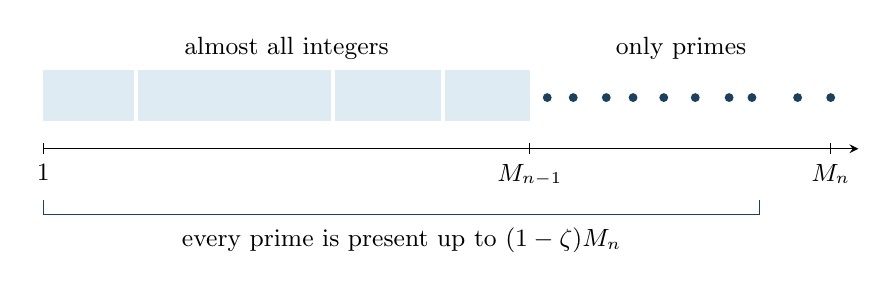
\begin{tikzpicture}[x=1cm,y=1cm,>=stealth,font=\small]
 \fill[paleblue] (0,0.35) rectangle (6.18,1.0);
 \foreach \x in {1.15,3.65,5.05}
   {\fill[white] (\x,0.35) rectangle (\x+0.055,1.0);}
 \foreach \x in {6.4,6.73,7.15,7.49,7.88,8.28,8.71,9.0,9.58,10}
   {\fill[inkblue] (\x,0.65) circle (1.6pt);}
 \draw[->] (0,0) -- (10.35,0);
 \draw (0,0.07) -- (0,-0.07) node[below] {$1$};
 \draw (6.18,0.07) -- (6.18,-0.07) node[below] {$M_{n-1}$};
 \draw (10,0.07) -- (10,-0.07) node[below] {$M_n$};
 \node at (3.09,1.28) {almost all integers};
 \node at (8.1,1.28) {only primes};
 \draw[inkblue] (0,-0.65) -- (0,-0.83) -- (9.1,-0.83) -- (9.1,-0.65);
 \node[below,align=center] at (4.55,-0.88)
   {every prime is present up to $(1-\zeta)M_n$};
\end{tikzpicture}
\caption{The eventual shape, schematically, for a fixed small $\zeta>0$.
The shaded region may have holes. Above $M_{n-1}$ every element is prime;
the theorem shows that the complete prime prefix approaches $M_n$.}
\label{fig:shape}
\end{figure}

The argument has three stages. Available primes first generate almost all
integers in a slightly smaller interval. Those integers then extend a
complete prime prefix at any fixed rate $\lambda<\ph$. Finally, if a
maximum lies a fixed proportion beyond that prefix, it supplies extra
representations and forces a definite increase of the prefix within a
bounded number of generations. A comparison with the Fibonacci upper
bound shows that such a discrepancy cannot persist.

All analytic facts needed for the last two stages are collected in
Section~\ref{sec:prime-tools}; the restricted representation lemma is
proved in Appendix~\ref{app:binary}. No theorem on almost-equal prime
summands is used. The relation with the accompanying Lean development is
described in Appendix~\ref{app:formal}.

\section{The elementary structure}
\label{sec:structure}

Throughout, $\N=\{1,2,\ldots\}$, $\Pp$ is the set of primes, and integer
counts in real intervals use their intersection with $\N$.
The sets $C_n$ are finite, nonempty, and increasing.

\begin{lemma}[Exhaustion]\label{lem:exhaustion}
Every finite initial segment of $\N$ is contained in some $C_n$.
In particular, $M_n\to\infty$.
\end{lemma}

\begin{proof}
We recall a short proof of the exhaustion result of \cite{CVZ}.
Induct on $m$. The case $m=1$ holds in $C_0$. Suppose $m\ge2$ and
$[1,m-1]\cap\N\subseteq C_j$.
If $m$ is prime, then $m=s((m-1)+1)\in C_{j+1}$.
If $m$ is composite, Bertrand's postulate gives a prime
$m-1<p\le2m-2$; since $m$ is not prime, $p>m$.
Both summands in
\[
 p=(m-1)+(p-m+1)
\]
belong to $[1,m-1]$, so $p\in C_{j+1}$. Also
$2\le2m-p\le m-1$, whence
\[
 m=s\bigl(p+(2m-p)\bigr)\in C_{j+2}.
\]
Here $2m$ is composite with least prime factor $2$. Retention completes
the induction. Since the maxima are increasing, exhaustion implies their
divergence.
\end{proof}

\begin{lemma}[The prime frontier and the Fibonacci bound]\label{lem:structure}
For $n\ge1$, the maximum $M_n$ is prime, and
\begin{equation}\label{eq:structure}
 C_n\subseteq\bigl([1,M_{n-1}]\cap\N\bigr)\cup\Pp.
\end{equation}
For $n\ge1$,
\begin{equation}\label{eq:fib-upper}
 M_{n+1}\le M_n+M_{n-1},\qquad M_n\le2M_{n-1}.
\end{equation}
\end{lemma}

\begin{proof}
If $a,b\le M_{n-1}$ and $a+b$ is composite, then
\[
 s(a+b)\le\frac{a+b}{2}\le M_{n-1}.
\]
Any new element above $M_{n-1}$ is therefore prime, proving
\eqref{eq:structure}. Since $M_1=2$, a maximum that increases becomes
prime, and a maximum that is retained remains prime. Moreover $M_2=3$,
so $M_n$ is odd for $n\ge2$.

For $n\ge2$, every even element of $C_n$ is at most $M_{n-1}$:
this follows from \eqref{eq:structure}, including the even prime $2$.
If $M_{n+1}>M_n$, it is an odd prime formed as the sum of an odd and
an even input from $C_n$. These are bounded by $M_n$ and $M_{n-1}$,
respectively. If the maximum is retained the same upper bound is immediate.
The case $n=1$ is $M_2=3=M_1+M_0$. Finally monotonicity gives
$M_n\le2M_{n-1}$ for $n\ge2$, and $M_1=2M_0$.
\end{proof}

We will compare prime cutoffs with a quantity that grows by at most an
exact factor $\ph$. Define
\begin{equation}\label{eq:weight}
 W_j=M_{j+1}+\frac{M_j}{\ph}.
\end{equation}
The coefficients are the positive left eigenvector of the Fibonacci matrix:
\[
 (1,\ph^{-1})\begin{pmatrix}1&1\\1&0\end{pmatrix}
 =\ph(1,\ph^{-1}).
\]
Consequently \eqref{eq:fib-upper} gives, for integers $j,r\ge0$,
\begin{equation}\label{eq:weight-growth}
 W_{j+1}\le\ph W_j,\qquad W_{j+r}\le\ph^rW_j.
\end{equation}
This weight removes the alternation between two consecutive maxima.

\section{The prime-representation tools}
\label{sec:prime-tools}

All logarithms are natural. The notation $f\ll g$ means that $|f|\le Cg$
for all sufficiently large scales; subscripts indicate permitted dependencies.
Write $f\sim g$ when $f/g\to1$, and $f=o(g)$ when $f/g\to0$.
All interval parameters below are fixed before the scale tends to infinity.

\begin{lemma}[Primes in proportional intervals]\label{lem:primes}
For fixed $0<\alpha<\beta$,
\[
 \#(\Pp\cap[\alpha X,\beta X])
 \sim\frac{(\beta-\alpha)X}{\log X},\qquad \pi(X)=o(X).
\]
For fixed $0<c<C$ and $w>0$, there is a constant $c_0>0$ such that,
uniformly for $a\in[c,C]$ and all sufficiently large $X$,
\begin{equation}\label{eq:moving-primes}
 \#(\Pp\cap[aX,(a+w)X])\ge c_0\frac X{\log X}.
\end{equation}
\end{lemma}

\begin{proof}
The first assertions follow by subtracting the prime number theorem at
$\alpha X$ and $\beta X$. For \eqref{eq:moving-primes}, choose a finite
grid of intervals of length $w/2$ such that every $[a,a+w]$, $a\in[c,C]$,
contains one grid interval. Apply the first assertion to this finite family,
taking the smallest positive lower-bound constant and the largest threshold.
Thus the width is fixed while the location may vary in a compact range.
\end{proof}

\begin{lemma}[Restricted binary representations]\label{lem:binary}
Fix $\nu\in\{1,2\}$, $0<\alpha<\beta$, $0<\gamma<d$, and
$\eta,B>0$. Set
\[
 I_X=[\alpha X,\beta X],\qquad J_X=[\gamma X,dX],\qquad
 \mathcal J_{\nu,X}(N)=\meas\{v\in I_X:N-\nu v\in J_X\}.
\]
Among integers $N$ satisfying
\begin{equation}\label{eq:binary-targets}
 1\le N\le BX,\qquad N\equiv\nu+1\pmod2,\qquad
 \mathcal J_{\nu,X}(N)\ge\eta X,
\end{equation}
all but $o(X/\log X)$ have a representation
\begin{equation}\label{eq:binary-representation}
 N=\nu p+q,\qquad p\in\Pp\cap I_X,\quad q\in\Pp\cap J_X.
\end{equation}
The exceptional bound depends only on the fixed displayed parameters.
\end{lemma}

The overlap $\mathcal J_{\nu,X}(N)$ measures how much of the line
$\nu v+w=N$ lies in the rectangle of allowed summands, with length
measured in the $v$ coordinate. Its positive proportional size keeps the
target away from a geometric obstruction. Parity is the local arithmetic
obstruction: for large $X$ both primes are odd.

Appendix~\ref{app:binary} proves the lemma for both coefficients together,
using the classical circle method. At every odd prime, multiplication by
$2$ is invertible, so the two cases have the same local factors. Their
factor at $2$ is also the same on the respective admissible parities.
The modern treatments of Helfgott \cite{Helfgott,HelfgottMinor} and Tao
\cite{Tao} explain the analytic framework; the actual estimates used in
the appendix are stated there explicitly.

The exceptional scale matters. Our candidate primes number
$\gg X/\log X$, and two sets of $o(X/\log X)$ exclusions cannot cover
them. An $o(X)$ bound alone would not suffice: a set of that size could
contain every prime candidate. The argument uses no claim that every
admissible target has a binary prime representation.

\section{Filling integers and propagating prime cutoffs}
\label{sec:filling}

For a real cutoff $L>0$, write
\[
 \Pref(j,L)\quad\Longleftrightarrow\quad
 \text{every prime }p\le L\text{ belongs to }C_j.
\]
Also let
\[
 H_j(Y)=\#\bigl(([1,Y]\cap\N)\setminus C_j\bigr)
\]
count missing integers. A prime cutoff measures complete coverage of primes;
the hole count measures approximate coverage of integers. They play different
roles. Lemma~\ref{lem:primes} implies, for every fixed $0<\rho<1$,
\begin{equation}\label{eq:prefix-max}
 \Pref(j,L)\quad\Longrightarrow\quad M_j\ge(1-\rho)L
\end{equation}
once $L$ is sufficiently large, with a threshold independent of $j$.

\begin{lemma}[Buffered filling]\label{lem:buffer}
For each fixed $0<\theta<1$, there is a function $e_\theta(X)\to0$
such that, uniformly in the generation $j$ and for all sufficiently large $X$,
\begin{equation}\label{eq:buffer}
 \Pref(j,X)\quad\Longrightarrow\quad
 H_{j+1}((1-\theta)X)\le e_\theta(X)\frac X{\log X}.
\end{equation}
\end{lemma}

\begin{proof}
The basic operation is averaging: if $2m=p+q$ with available primes and
$m\ge2$, then $s(p+q)=m$.
At a scale $Y$, take both prime intervals to be $[a,Y]$, where
$a=(1-\theta)Y/4$. For
\[
 (1-\theta)Y/2\le m\le(1-\theta)Y,
\]
the overlap of $[a,Y]$ and $[2m-Y,2m-a]$ has length
\[
 \min(2m-2a,\,2Y-2m,\,Y-a)
 \ge\eta_\theta Y,\qquad
 \eta_\theta=\min((1-\theta)/2,2\theta)>0.
\]
Lemma~\ref{lem:binary} with $\nu=1$ and $B=2$ therefore leaves at most
$e(Y)Y/\log Y$ exceptional midpoints, for some nonnegative $e(Y)\to0$.
All other midpoints are generated once every prime at most $Y$ is present.

Apply this at $Y_r=X/2^r$ for all $r\ge0$ with $Y_r\ge\sqrt X$.
The midpoint intervals are adjacent and cover
$[\sqrt X,(1-\theta)X]$, apart from a possible bottom interval of
length $O(\sqrt X)$. Indeed the last scale is less than $2\sqrt X$.
Moreover $\sum_rY_r\le2X$ and $\log Y_r\ge\frac12\log X$, so the
total number of exceptions is at most
\[
 4\sup_{Y\ge\sqrt X}e(Y)\frac X{\log X}
 =o(X/\log X).
\]
The omitted bottom range has the same negligible size. Every prime used
lies below $X$, and the exceptional estimate is independent of $j$.
\end{proof}

The buffer is fixed. We never replace $\theta$ by an unspecified function
of $X$; it is allowed to tend to zero only after the limiting estimates
have been proved for each fixed value.

\begin{lemma}[Extension of a prime cutoff]\label{lem:extension}
Fix $0<\epsilon<1$ and $B\ge1$. For all sufficiently large $Y$, if
$Y\le X\le BY$, $\Pref(j,Y)$, and $\Pref(j+1,X)$, then
\begin{equation}\label{eq:extension}
 \Pref\bigl(j+2,(1-\epsilon)(X+Y)\bigr).
\end{equation}
\end{lemma}

\begin{proof}
Only a prime $r$ with $X<r\le(1-\epsilon)(X+Y)$ needs attention.
For every prime $p\in[(1-\epsilon)X,X]$, the complement $a=r-p$ is
positive and satisfies $a\le(1-\epsilon)Y$. Distinct primes give
distinct complements. Lemma~\ref{lem:primes} supplies
$\gg_\epsilon X/\log X$ candidates; Lemma~\ref{lem:buffer} leaves only
$o(Y/\log Y)=o(X/\log X)$ missing complements in $C_{j+1}$.
The comparison is uniform for $Y\le X\le BY$.
Some candidate therefore has both $p,a\in C_{j+1}$, and
$s(p+a)=r\in C_{j+2}$. Smaller primes are retained.
\end{proof}

Fix $8/5\le\lambda<\ph$ and put
\begin{equation}\label{eq:epsilon}
 \epsilon=1-\frac{\lambda^2}{\lambda+1},
 \qquad \lambda^2=(1-\epsilon)(\lambda+1).
\end{equation}
Then $0<\epsilon<1$. We call $(j,L)$ a \emph{prime profile} if
\begin{equation}\label{eq:profile}
 \Pref(j,L)\quad\text{and}\quad\Pref(j+1,\lambda L).
\end{equation}
This is just a pair of complete prime cutoffs in consecutive generations.
For sufficiently large $L$, Lemma~\ref{lem:extension} advances a profile
from $(j,L)$ to $(j+1,\lambda L)$. Iteration gives profiles
$(j+r,\lambda^rL)$ for every $r\ge0$. We call this ordinary propagation.

\section{An outlying prime forces an increase}
\label{sec:boost}

Ordinary propagation runs at rate $\lambda<\ph$. To show that its cutoffs
nevertheless approach the true maxima, we need a way to increase a profile
when the maximum is substantially ahead. An available prime beyond the
cutoff supplies precisely this mechanism.

\begin{lemma}[Increase of a prime profile]\label{lem:boost}
Fix $0<\delta\le1/10$ and $8/5\le\lambda<\ph$, with $\epsilon$ as in
\eqref{eq:epsilon}. Define
\begin{equation}\label{eq:boost-parameters}
 w=\frac\delta{20},\qquad b=\frac\delta8,\qquad
 \kappa=\frac{(1-\epsilon)b}{\lambda^4}>0.
\end{equation}
There is a threshold $L_0$, independent of $j$, such that any prime profile
$(j,L)$ with $L\ge L_0$ and $M_j>(1+\delta)L$ produces a profile
\begin{equation}\label{eq:boosted-profile}
 \bigl(j+3,(1+\kappa)\lambda^3L\bigr).
\end{equation}
\end{lemma}

\begin{proof}
\emph{Choose an available prime of controlled size.}
Let $i$ be the first index with $M_i>(1+\delta)L$. For large $L$,
$1\le i\le j$. By Lemma~\ref{lem:structure} and retention,
\begin{equation}\label{eq:outlier}
 t=M_i\in C_j\cap\Pp,\qquad
 1+\delta<\tau:=t/L\le2+2\delta.
\end{equation}
The upper bound uses $M_i\le2M_{i-1}$, and $t$ is odd since $t>2$.

\emph{Generate almost every prime in an extra interval.}
Use the source intervals
\begin{equation}\label{eq:boost-source}
 I=[\lambda-w,\lambda]L,\qquad J=[1-4w,1]L
\end{equation}
and the target interval
\begin{equation}\label{eq:boost-target}
 U=\left[\lambda+\frac{\tau+1}{2}-2w,
          \lambda+\frac{\tau+1}{2}-w\right]L.
\end{equation}
Every prime in $I$ belongs to $C_{j+1}$, and every prime in $J$ belongs
to $C_j$. These intervals have positive endpoints.

For every real $p\in I$ and $u\in U$, endpoint subtraction gives
\begin{equation}\label{eq:boost-overlap}
 2u-t-2p\in[(1-4w)L,L]=J.
\end{equation}
Thus the real overlap for the equation $2p+q=2u-t$ has length $wL$.
If $u$ is an integer, the target $2u-t$ is odd, and
\[
 2u-t\in[(2\lambda+1-4w)L,(2\lambda+1-2w)L]\subset[1,6L]
\]
for large $L$. Notice that this target range and both source intervals
are independent of $t$. Lemma~\ref{lem:binary} with $\nu=2$ therefore
applies with one exceptional set at scale $L$. Since $u\mapsto2u-t$ is
injective, all but $o(L/\log L)$ integers $u\in U$ have the required
representation, uniformly in the chosen $j,t$.

For each such $u$ that is prime, the operations are
\begin{equation}\label{eq:boost-operations}
 \frac{t+q}{2}=s(t+q)\in C_{j+1},\qquad
 u=p+\frac{t+q}{2}=s\left(p+\frac{t+q}{2}\right)\in C_{j+2}.
\end{equation}
The first sum is even and composite; the second is the prime $u$.
It follows that
\begin{equation}\label{eq:extra-primes}
 \#\bigl((\Pp\cap U)\setminus C_{j+2}\bigr)=o(L/\log L).
\end{equation}

\emph{Turn the extra primes into a complete larger cutoff.}
Ordinary propagation already gives every prime at most $\lambda^3L$
in $C_{j+3}$. Take a prime
$r\in(\lambda^3L,(\lambda^3+b)L]$ and consider $v=r-u$ for $u\in U$.
The needed margin is
\begin{equation}\label{eq:complement-margin}
 \frac45L\le v\le(\lambda-11\delta/40)L
       <(\lambda-\delta/4)L.
\end{equation}
Here is the complete calculation. Since $x^3-2x-1$ is increasing on
$[8/5,\ph]$ and vanishes at $\ph$,
\begin{align*}
 v/L
 &\le\lambda^3-\lambda+b-(\tau+1)/2+2w\\
 &\le\lambda+b-\delta/2+2w
 =\lambda-11\delta/40.
\end{align*}
For the lower bound, $\lambda^3-\lambda\ge12/5$ on the same interval,
while $(\tau+1)/2\le8/5$. Hence
\[
 v/L\ge\lambda^3-\lambda-(\tau+1)/2+w\ge4/5.
\]

Apply buffered filling at prime cutoff $\lambda L$ in $C_{j+1}$, with
$\theta=\delta/(4\lambda)$. Only $o(L/\log L)$ integers up to
$(\lambda-\delta/4)L$ are missing from $C_{j+2}$.
Meanwhile $U$ has length $wL$ and its left endpoint stays in a fixed
compact interval of positive multiples of $L$, by \eqref{eq:outlier}.
The uniform form \eqref{eq:moving-primes} supplies $\gg L/\log L$
candidate primes in $U$.

Exclude those absent from $C_{j+2}$, using \eqref{eq:extra-primes}, and
those whose complement $r-u$ is absent. The latter exclusion is at most
the buffered hole count, since $u\mapsto r-u$ is injective.
The total is $o(L/\log L)$, so a candidate remains. Its two available
inputs generate the prime $r$ in $C_{j+3}$. All bounds are uniform in
$r,j,t$, proving
\begin{equation}\label{eq:improved-cutoff}
 \Pref(j+3,(\lambda^3+b)L).
\end{equation}

\emph{Rebalance the two consecutive cutoffs.}
At time $j+2$ the ordinary cutoff is $\lambda^2L$. The ratio
$(\lambda^3+b)/\lambda^2$ lies between $1$ and $2$ throughout our
parameter range. Applying Lemma~\ref{lem:extension} once more gives
the cutoff
\[
 (1-\epsilon)(\lambda^3+b+\lambda^2)L
 =\bigl(\lambda^4+(1-\epsilon)b\bigr)L
 =(1+\kappa)\lambda^4L
\]
in $C_{j+4}$. The cutoff in \eqref{eq:improved-cutoff} is at least
$(1+\kappa)\lambda^3L$, because
$\kappa\lambda^3=(1-\epsilon)b/\lambda\le b$.
These are the two cutoffs required by \eqref{eq:boosted-profile}.
\end{proof}

The generations in the central construction are worth keeping visible:
\begin{center}
\begin{tabular}{@{}cl@{}}
\toprule
Generation & Available quantities or newly generated output\\
\midrule
$j$ & The outlying prime $t$ and source primes $q\in J$\\
$j+1$ & The average $(t+q)/2$ and source primes $p\in I$\\
$j+2$ & Almost every prime $u=p+(t+q)/2$ in $U$\\
$j+3$ & Every prime in the enlarged cutoff, using $r=u+(r-u)$\\
$j+4$ & A second cutoff that restores the profile's ratio $\lambda$\\
\bottomrule
\end{tabular}
\end{center}
The two exceptional sets are small compared with the candidate primes.
This is what converts almost-all representations into a complete prime cutoff.

\begin{samepage}
\section{Why the prime cutoffs catch the maxima}
\label{sec:comparison}

We first isolate the sequence argument. An ordinary step may increase a
discrepancy slightly. If a large discrepancy forces a definite contraction
within four steps, the discrepancy is eventually small at every step.

\begin{lemma}[Comparison over boundedly many steps]\label{lem:comparison}
Let $\lambda>1$, $A\ge1$, $\kappa>0$, and $T>0$, with
$\rho=A^4/(1+\kappa)<1$.
Let $\mathcal A$ be a nonempty family of pairs $(j,L)$, where
$j\ge0$ is an integer and $L>0$, and let $Z:\mathcal A\to(0,\infty)$.
Suppose:
\begin{enumerate}[label=\textup{(\roman*)}]
\item Each $(j,L)\in\mathcal A$ has $(j+1,\lambda L)\in\mathcal A$ and
$Z(j+1,\lambda L)\le A Z(j,L)$.
\item If $Z(j,L)>T$, then for some $h\in\{3,4\}$ the pair
$(j+h,(1+\kappa)\lambda^hL)$ is in $\mathcal A$, and its $Z$-value is
at most $A^hZ(j,L)/(1+\kappa)$.
\end{enumerate}
Then for every sufficiently large integer $n$ there is $(n,L_n)\in\mathcal A$
such that
\begin{equation}\label{eq:abstract-comparison}
 L_n\longrightarrow\infty,\qquad Z(n,L_n)\le A^4T.
\end{equation}
\end{lemma}
\end{samepage}

\begin{proof}
Starting from any admissible pair, select successive pairs as follows:
take an ordinary step when $Z\le T$, and a step from (ii) when $Z>T$.
The selected indices increase by integers between $1$ and $4$.
Some selected pair has $Z\le T$; otherwise repeated contraction would
give $Z_m\le\rho^mZ_0\to0$, contrary to $Z_m>T$.
After the first such pair, every selected pair satisfies $Z\le AT$.
Indeed an ordinary step starts at $Z\le T$, and a step of type (ii)
contracts the preceding bound.

Between consecutive selected indices $j$ and $j+h$, use ordinary
propagation from the earlier selected pair. At an intermediate index
$j+r$, $0\le r<h\le4$, the resulting value is at most
$A^r(AT)\le A^4T$. This covers every sufficiently large integer index.
The corresponding scales increase by at least $\lambda$ per elapsed
generation, including the transitions to selected pairs, and hence diverge.
\end{proof}

\begin{proposition}[Approximate prime completeness]\label{prop:complete}
For every fixed $0<\zeta<1$, $\Pref(n,(1-\zeta)M_n)$ holds for all
sufficiently large $n$.
\end{proposition}

\begin{proof}
Fix $0<\delta\le1/10$. As $\lambda\uparrow\ph$ in
\eqref{eq:epsilon}--\eqref{eq:boost-parameters},
\[
 A:=\ph/\lambda\longrightarrow1,\qquad
 \epsilon\longrightarrow0,\qquad
 \kappa\longrightarrow\frac{\delta}{8\ph^4}>0.
\]
By continuity, we may fix $8/5\le\lambda<\ph$ sufficiently close to
$\ph$ that
\begin{equation}\label{eq:choose-lambda}
 A^4<1+\delta,\qquad \frac{A^4}{1+\kappa}<1.
\end{equation}
All parameters are now fixed before any scale tends to infinity.

Take $L_*$ beyond the thresholds for ordinary propagation, the profile
increase, and \eqref{eq:prefix-max} with accuracy $\delta$.
Let $\mathcal A$ be the prime profiles $(j,L)$ with $L\ge L_*$.
This family is nonempty by exhaustion: a generation containing every
integer up to $\ceil{\lambda L_*}$ supplies a profile at cutoff $L_*$.
For a profile define the relative discrepancy
\begin{equation}\label{eq:discrepancy}
 Z(j,L)=\frac{W_j}{(\lambda+\ph^{-1})L}
       =\frac{M_{j+1}+M_j/\ph}{(\lambda+\ph^{-1})L}.
\end{equation}
The denominator is the same Fibonacci weight applied to the profile's
two cutoffs. By \eqref{eq:weight-growth}, ordinary propagation gives
$Z(j+1,\lambda L)\le A Z(j,L)$.

If $Z(j,L)>1+\delta$, at least one of
\[
 M_j>(1+\delta)L,\qquad M_{j+1}>(1+\delta)\lambda L
\]
must hold. In the first case Lemma~\ref{lem:boost} increases the profile
after three steps. In the second, first propagate ordinarily and then
apply that lemma, giving an increase after four steps.
For the resulting $h\in\{3,4\}$, \eqref{eq:weight-growth} shows
\[
 Z\bigl(j+h,(1+\kappa)\lambda^hL\bigr)
 \le\frac{A^h}{1+\kappa}Z(j,L).
\]
Thus Lemma~\ref{lem:comparison}, with $T=1+\delta$, applies.
For every sufficiently large $n$ there is a profile $(n,L_n)$ with
$L_n\to\infty$ and
\begin{equation}\label{eq:close-weight}
 Z(n,L_n)\le A^4(1+\delta)\le(1+\delta)^2.
\end{equation}

The second cutoff of this profile gives
$M_{n+1}\ge(1-\delta)\lambda L_n$ by \eqref{eq:prefix-max}.
Solving \eqref{eq:close-weight} for the other maximum gives
\begin{align*}
 \frac{M_n}{L_n}
 &\le(1+\delta)^2(\ph\lambda+1)-(1-\delta)\ph\lambda\\
 &=1+(2\delta+\delta^2)(\ph\lambda+1)+\delta\ph\lambda
 =1+O(\delta).
\end{align*}
The constant is absolute, since $\lambda\le\ph$ and $\delta\le1/10$.
In particular it can be taken to be $12$. Given $\zeta$, choose
$\delta>0$ small enough that $(1+12\delta)^{-1}\ge1-\zeta$.
Since the profile contains every prime up to $L_n$, the desired
prime completeness follows.
\end{proof}

\section{The limits}
\label{sec:limits}

\begin{proof}[Proof of Theorem~\ref{thm:main}]
\emph{The Fibonacci bound is asymptotically attained.}
Fix $0<\zeta<1$. By Proposition~\ref{prop:complete}, for all large $n$
the consecutive generations have prime cutoffs
\[
 Y=(1-\zeta)M_{n-1},\qquad X=(1-\zeta)M_n,
 \qquad Y\le X\le2Y.
\]
Lemma~\ref{lem:extension} with $\epsilon=\zeta$ puts every prime up to
$(1-\zeta)^2(M_n+M_{n-1})$ in $C_{n+1}$.
Using \eqref{eq:prefix-max} at this cutoff, together with the upper bound,
we obtain
\[
 (1-\zeta)^3(M_n+M_{n-1})\le M_{n+1}\le M_n+M_{n-1}.
\]
Since $\zeta$ is arbitrary,
\begin{equation}\label{eq:saturation}
 \frac{M_{n+1}}{M_n+M_{n-1}}\longrightarrow1.
\end{equation}

\emph{The maximum ratio converges.}
Set $r_n=M_{n+1}/M_n$. Monotonicity and \eqref{eq:fib-upper} give
$1\le r_n\le2$. Equation~\eqref{eq:saturation} implies
\[
 r_n=1+\frac1{r_{n-1}}+e_n,\qquad e_n\longrightarrow0.
\]
Indeed the multiplier $1+1/r_{n-1}$ relating the two errors is at most $2$.
Since $\ph=1+1/\ph$,
\[
 |r_n-\ph|\le\frac{|r_{n-1}-\ph|}{\ph r_{n-1}}+|e_n|
 \le\ph^{-1}|r_{n-1}-\ph|+|e_n|.
\]
The finite number $D=\limsup_n|r_n-\ph|$ therefore satisfies
$D\le\ph^{-1}D$, so $D=0$ and $r_n\to\ph$.

\emph{The preceding maximum determines the cardinality.}
Again fix $0<\zeta<1$. Prime completeness at time $n-1$ and buffered
filling with $\theta=\zeta$ give
\[
 H_n((1-\zeta)^2M_{n-1})=o(M_{n-1}/\log M_{n-1}).
\]
Hence $\liminf_n|C_n|/M_{n-1}\ge(1-\zeta)^2$.
On the other hand, the prime-frontier inclusion \eqref{eq:structure} gives
\[
 |C_n|\le M_{n-1}+\pi(M_n)
 \le M_{n-1}+\pi(2M_{n-1})=M_{n-1}+o(M_{n-1}).
\]
Letting $\zeta\downarrow0$ proves $|C_n|/M_{n-1}\to1$.
The remaining limits follow from
\[
 \frac{|C_{n+1}|}{|C_n|}
 =\frac{|C_{n+1}|}{M_n}\frac{M_n}{M_{n-1}}
       \left(\frac{|C_n|}{M_{n-1}}\right)^{-1},\qquad
 \frac{|C_n|}{M_n}=\frac{|C_n|}{M_{n-1}}\frac{M_{n-1}}{M_n}.
\]
\end{proof}

\begin{remark}[Complete primes, approximate integers]
Let $Q_n$ be the largest prime such that every prime at most $Q_n$ belongs
to $C_n$; it is well-defined for $n\ge1$. The theorem and
Lemma~\ref{lem:primes} imply $Q_n/M_n\to1$: for each fixed $\zeta>0$,
there is eventually a prime between $(1-\zeta)^2M_n$ and
$(1-\zeta)M_n$, and that prime is at most $Q_n$.
For integers the conclusion is approximate coverage below $M_{n-1}$:
\[
 H_n(M_{n-1})\le M_{n-1}-|C_n|+\pi(M_n)=o(M_{n-1}).
\]
It does not assert that this entire interval is present.
\end{remark}

\begin{remark}[Ratio convergence and amplitude]
The theorem proves the ratio limits without asserting that $M_n/\ph^n$
has a positive limit. Such an amplitude conclusion requires additional
control of accumulated errors. For example,
$x_n=\ph^n/(n+3)$ is increasing, satisfies
$x_{n+1}\le x_n+x_{n-1}$ for $n\ge1$, and has
$x_{n+1}/(x_n+x_{n-1})\to1$, while $x_n/\ph^n\to0$.
To check the inequality, set $m=n+3$ and compute
\[
 \frac{x_n+x_{n-1}-x_{n+1}}{x_n}
 =\frac1{\ph(m-1)}+\frac\ph{m+1}>0.
\]
The comparison argument above uses a fixed improvement when a gap is
present; it does not sum relative errors over infinitely many generations.
\end{remark}

\appendix
\section{The restricted binary representation lemma}\label{app:binary}

We prove Lemma~\ref{lem:binary} simultaneously for $\nu=1$ and $\nu=2$.
The interval ratios $\alpha,\beta,\gamma,d$, the overlap margin
$\eta>0$, and the target bound $B>0$ remain fixed throughout. Constants
may depend on these parameters. The proof gives the stronger exceptional
bound $O(X/\log^4 X)$.

The argument is the classical circle method: the major arcs supply a
positive main term, and a mean-square estimate makes the minor arcs small
for almost every target. Helfgott's account of the ternary Goldbach
problem~\cite{Helfgott} provides a modern perspective on this method.
The analytic inputs used here are the two standard estimates stated
below; the restricted binary conclusion is proved here.

\subsection{The two analytic inputs and the weighted count}

Write $e(z)=\exp(2\pi iz)$, let $\Lambda$ be the von Mangoldt function,
let $\mu$ be the M\"obius function, and write $\tot$ for Euler's totient.
We use Siegel--Walfisz in the form
\begin{equation}\label{app:sw}
 \sum_{\substack{n\le x\\n\equiv a\pmod q}}\Lambda(n)
 =\frac{x}{\tot(q)}+O_{D,E}\left(\frac{x}{\log^D x}\right),
 \qquad (a,q)=1,\quad q\le(\log x)^E,
\end{equation}
for every fixed $D,E>0$ and $x\ge2$. Its constants may be ineffective.
Here $q$ is a positive integer and $a$ is a coprime residue class.
We also use the classical Vaughan estimate
\begin{equation}\label{app:vaughan}
 \left|\sum_{p\le x}(\log p)e(p\theta)\right|
 \ll(\log x)^4
 \left(\frac{x}{\sqrt q}+x^{4/5}+\sqrt{xq}\right),
 \quad
 \left|\theta-\frac aq\right|\le q^{-2},\quad
 (a,q)=1,\quad 1\le q\le x,
\end{equation}
for $x\ge2$. These are standard circle-method inputs; see
\cite[Theorem~3.1]{Vaughan} and the major-arc discussion in
\cite[Proposition~24]{Tao}. No explicit numerical constants are needed.

The case $q=1$ of \eqref{app:sw} gives
$\sum_{n\le x}\Lambda(n)=x+O_D(x/\log^D x)$.
Proper prime powers contribute $O(\sqrt x\log^2 x)$: sum over at most
$\log_2x$ exponents, at most $\sqrt x$ bases for each exponent, and
weight at most $\log x$ for each term. Consequently
\begin{equation}\label{app:theta}
 \vartheta(x):=\sum_{p\le x}\log p
 =x+O_D(x/\log^D x),\qquad \vartheta(x)\ll x.
\end{equation}
Here and below sums indexed by $p$ are over primes. Adding proper
prime powers to \eqref{app:vaughan} gives the same bound for the
von Mangoldt sum, since their contribution is absorbed by its
$x^{4/5}(\log x)^4$ term.
Partial summation also gives
\[
 \pi(x)=\frac{\vartheta(x)}{\log x}
       +\int_2^x\frac{\vartheta(t)}{t\log^2t}\,dt
 =\frac{x}{\log x}+O(x/\log^2x).
\]
For the integral estimate, split at $\sqrt x$ and use
$\vartheta(t)\ll t$. Thus the prime number theorem used in
Lemma~\ref{lem:primes} follows from the same analytic input.

Put $I_X=[\alpha X,\beta X]$, $J_X=[\gamma X,dX]$, and
\[
 S_I(\theta)=\sum_{p\in I_X}\log p\,e(p\theta),\qquad
 S_J(\theta)=\sum_{p\in J_X}\log p\,e(p\theta).
\]
Fourier orthogonality gives the exact identity
\begin{equation}\label{app:count}
 \begin{aligned}
 R_X(N)&:=\int_0^1 S_I(\nu\theta)S_J(\theta)e(-N\theta)\,d\theta\\
 &=\sum_{\substack{p\in\Pp\cap I_X,\ r\in\Pp\cap J_X\\\nu p+r=N}}
                  (\log p)(\log r).
 \end{aligned}
\end{equation}
Thus $R_X(N)>0$ is equivalent to the required prime representation.

\subsection{Minor arcs: a mean-square bound}

Fix $P=(\log X)^{20}$. Around each reduced fraction $a/q$ with
$q\le P$, take the arc of radius $P/X$ on $\R/\Z$; include $0/1$.
Their union is $\mathfrak M$, and its complement is $\mathfrak m$.
Distinct fractions are at circular distance at least $P^{-2}$, so
the arcs are disjoint for large $X$, and
$\meas(\mathfrak M)\ll P^3/X$.
Write $R_{\mathfrak M}(N)$ and $R_{\mathfrak m}(N)$ for the two
parts of the integral in \eqref{app:count}.

Dirichlet approximation with denominator bound $\ceil{X/P}$ gives,
for every $\theta\in\mathfrak m$, a reduced fraction $a/q$ with
\[
 P<q\le2X/P,\qquad
 \left|\theta-a/q\right|\le q^{-2}.
\]
Indeed the approximation error is at most $P/(qX)$; a denominator
$q\le P$ would therefore put $\theta$ in $\mathfrak M$.
Distances can be interpreted modulo one by changing $a$ by a multiple
of $q$.

Apply \eqref{app:vaughan} to the two initial sums defining $S_J$.
Their endpoints are fixed positive multiples of $X$, and hence exceed
$2X/P$ for large $X$. Changing an endpoint convention costs
$O(\log X)$, which is absorbed below. We obtain
\begin{equation}\label{app:minor-sup}
 \sup_{\theta\in\mathfrak m}|S_J(\theta)|
 \ll XP^{-1/2}(\log X)^4+X^{4/5}(\log X)^4.
\end{equation}
Also, by orthogonality and \eqref{app:theta},
\[
 \int_0^1|S_I(\nu\theta)|^2\,d\theta
 =\sum_{p\in I_X}(\log p)^2\ll X\log X.
\]
Multiplication of the frequencies by the nonzero integer $\nu$ does
not affect this identity. Bessel's inequality now gives
\begin{align}
 \sum_{N\in\Z}|R_{\mathfrak m}(N)|^2
 &\le\int_{\mathfrak m}|S_I(\nu\theta)S_J(\theta)|^2\,d\theta
 \notag\\
 &\ll X^3P^{-1}(\log X)^9+X^{13/5}(\log X)^9
 \ll\frac{X^3}{\log^4 X}.\label{app:minor-square}
\end{align}
The last step uses $P=(\log X)^{20}$ and
$X^{-2/5}(\log X)^{13}\to0$.
For every fixed $c>0$, it follows that
\begin{equation}\label{app:minor-exceptions}
 \#\{N\in\Z:|R_{\mathfrak m}(N)|>cX\}
 \ll_c X/\log^4X.
\end{equation}
This is the point where averaging over targets replaces a bound for
each individual binary representation problem.

\subsection{Major arcs and the real overlap}

For an interval $K$, write $V_K(\zeta)=\int_K e(v\zeta)\,dv$.
On the arc $\theta=a/q+\zeta$, put
$q_\nu=q/(q,\nu)$, the denominator of the reduced fraction $\nu a/q$.
For every fixed $H>0$, Siegel--Walfisz and partial summation give
uniformly on all these arcs
\begin{equation}\label{app:major-approx}
 \begin{aligned}
 S_J(a/q+\zeta)
  &=\frac{\mu(q)}{\tot(q)}V_{J_X}(\zeta)
       +O_H(X/\log^H X),\\
 S_I(\nu a/q+\nu\zeta)
  &=\frac{\mu(q_\nu)}{\tot(q_\nu)}V_{I_X}(\nu\zeta)
       +O_H(X/\log^H X).
 \end{aligned}
\end{equation}
For completeness, decompose a von Mangoldt sum into residue classes
modulo its reduced denominator. On each coprime class,
\eqref{app:sw} and partial summation replace the sum by its integral
with density $1/\tot(q)$, with error
$O(X(1+X|\zeta|)/\log^D X)$.
All intermediate endpoints lie in $[cX,CX]$ for fixed $0<c<C$,
so \eqref{app:sw} applies uniformly with any fixed modulus exponent
greater than $20$. Summing the errors over at most $P$ classes costs
at most $O(P^2X/\log^D X)$. The main coefficients sum to
$\sum_{(b,q)=1}e(ab/q)=\mu(q)$.
The total von Mangoldt weight in noncoprime classes is
$O(\log(2q)\log X)$, since it is supported on powers of primes
dividing $q$. Removing all proper prime powers costs
$O(\sqrt X\log^2X)$. Taking $D$ sufficiently large in terms of $H$
absorbs these errors. The same argument applies with denominator
$q_\nu$ and frequency $\nu\zeta$, proving both formulas.

Define
\[
 c_q(N)=\sum_{\substack{0\le a<q\\(a,q)=1}}e(-Na/q),\qquad
 w_\nu(q)=\frac{\mu(q)\mu(q_\nu)}{\tot(q)\tot(q_\nu)},
\]
\[
 \mathfrak S_{\nu,P}(N)=\sum_{q\le P}w_\nu(q)c_q(N).
\]
The sums and integrals in \eqref{app:major-approx} are $O(X)$, by
\eqref{app:theta}. Multiply those formulas and integrate over
$\mathfrak M$. Choosing $H$ so that
$P^3/\log^H X\le1/\log^4X$ gives
\begin{equation}\label{app:major-truncated}
 R_{\mathfrak M}(N)
 =\mathfrak S_{\nu,P}(N)
    \int_{-P/X}^{P/X}
      V_{I_X}(\nu\zeta)V_{J_X}(\zeta)e(-N\zeta)\,d\zeta
   +O(X/\log^4X).
\end{equation}
This error is uniform in $N$.

For any interval $K$ and nonzero $\zeta$,
$|V_K(\zeta)|\le\min(\meas(K),1/(\pi|\zeta|))$.
Therefore extending the last integral to $\R$ costs $O(X/P)$.
If $w_\nu(q)\ne0$, then $q$ is squarefree, and
$\tot(q_\nu)=\tot(q)$: for $\nu=2$, removing a single factor $2$
does not change the totient. Thus
\begin{equation}\label{app:coefficient-bound}
 |w_\nu(q)|\le\tot(q)^{-2},\qquad
 \sum_{q\le P}|w_\nu(q)c_q(N)|
 \le\sum_{q\le P}\frac1{\tot(q)}\ll\log^2(2P).
\end{equation}
For the last bound, $q/\tot(q)\le\tau(q)$ prime by prime, where
$\tau$ counts divisors, and
$\sum_{q\le P}\tau(q)/q=\sum_{ab\le P}1/(ab)\le(1+\log P)^2$.
Hence the total integral-tail error is
$O(X\log^2(2P)/P)=O(X/\log^4X)$.

The full integral is exactly the overlap in Lemma~\ref{lem:binary}.
Indeed the continuous function
\[
 f(y)=\left(\nu^{-1}\ind_{\nu I_X}*\ind_{J_X}\right)(y)
     =\int_{I_X}\ind_{J_X}(y-\nu v)\,dv
\]
has Fourier transform $V_{I_X}(\nu\zeta)V_{J_X}(\zeta)$, using the
positive-exponential convention. This transform is integrable by
the preceding bound. Fourier inversion therefore gives
\[
 \int_\R V_{I_X}(\nu\zeta)V_{J_X}(\zeta)e(-N\zeta)\,d\zeta
 =f(N)=\mathcal J_{\nu,X}(N).
\]
Consequently
\begin{equation}\label{app:major-final}
 R_{\mathfrak M}(N)
 =\mathfrak S_{\nu,P}(N)\mathcal J_{\nu,X}(N)
      +O(X/\log^4X),
\end{equation}
uniformly in the targets.

\subsection{An averaged bound for the singular-series tail}

We give an elementary estimate that avoids detailed divisor-function
bounds. Put $f_0(n)=(n/\tot(n))^2$. Define a nonnegative multiplicative
function $g$, supported on squarefree integers, by
\[
 g(\ell)=\left(\frac{\ell}{\ell-1}\right)^2-1
       =\frac{2\ell-1}{(\ell-1)^2}
\]
at every prime $\ell$. Then
$f_0(n)=\sum_{d\mid n}g(d)$, and
\[
 G:=\sum_{d\ge1}\frac{g(d)}d
   =\prod_\ell\left(1+\frac{g(\ell)}\ell\right)<\infty,
\]
because $g(\ell)/\ell=O(\ell^{-2})$.
Interchanging nonnegative sums yields, for $x\ge1$,
\begin{equation}\label{app:totient-means}
 \begin{aligned}
 \sum_{n\le x}f_0(n)&\le Gx,\\
 \sum_{n\le x}\frac{f_0(n)}n
 &=\sum_{d\le x}\frac{g(d)}d\sum_{k\le x/d}\frac1k
 \le G(1+\log x).
 \end{aligned}
\end{equation}
Dyadic summation of the first bound gives
\[
 \sum_{k>z}\frac1{\tot(k)^2}
 =\sum_{k>z}\frac{f_0(k)}{k^2}\ll z^{-1}\qquad(z\ge1).
\]
The full sum is finite, so after enlarging the constant this bound
also holds for $0<z<1$.

M\"obius inversion in the definition of $c_q(N)$ gives
\[
 c_q(N)=\sum_{h\mid(q,N)}h\mu(q/h),\qquad
 |c_q(N)|\le\sum_{h\mid(q,N)}h.
\]
The totient product formula gives
$\tot(hk)\ge\tot(h)\tot(k)$. Thus for $Y\ge1$ and $N\ge1$,
\begin{align}
 \sum_{q>Y}\frac{|c_q(N)|}{\tot(q)^2}
 &\le\sum_{h\mid N}\frac{h}{\tot(h)^2}
                 \sum_{k>Y/h}\frac1{\tot(k)^2}
 \notag\\
 &\ll\frac1Y F(N),\qquad
 F(N):=\sum_{h\mid N}f_0(h).\label{app:series-tail}
\end{align}
In particular these series converge absolutely for each fixed $N$.
Their average is controlled by \eqref{app:totient-means}:
\begin{equation}\label{app:F-mean}
 \sum_{1\le N\le BX}F(N)
 =\sum_{h\le BX}f_0(h)\floor{\frac{BX}{h}}
 \le BX\sum_{h\le BX}\frac{f_0(h)}h
 \ll_B X\log X.
\end{equation}

\subsection{Local factors and completion}

Absolute convergence permits the Euler-product evaluation of
\[
 \mathfrak S_\nu(N)=\sum_{q\ge1}w_\nu(q)c_q(N).
\]
Both factors in the summand are multiplicative in $q$.
For $w_\nu$, this follows from its explicit squarefree formula:
$w_1(q)=\mu(q)^2/\tot(q)^2$, while $w_2(q)$ is this same expression
with its sign reversed when $q$ is even. For $c_q(N)$ it follows
from the Chinese remainder theorem, or its divisor formula above.
At an odd prime $\ell$, the local factor is, for either $\nu$,
\[
 1+\frac{c_\ell(N)}{(\ell-1)^2},\qquad
 c_\ell(N)=
 \begin{cases}
 \ell-1,&\ell\mid N,\\
 -1,&\ell\nmid N.
 \end{cases}
\]
At $2$, the factor is $1+c_2(N)$ for $\nu=1$, and $1-c_2(N)$
for $\nu=2$. It equals $2$ in both cases when
$N\equiv\nu+1\pmod2$. On that parity, therefore,
\begin{equation}\label{app:singular-positive}
 \begin{aligned}
 \mathfrak S_\nu(N)
 &=2C_2\prod_{\substack{\ell\mid N\\\ell>2}}
                 \frac{\ell-1}{\ell-2}
 \ge s_0:=2C_2>0,\\
 C_2&:=\prod_{\ell>2}\left(1-\frac1{(\ell-1)^2}\right).
 \end{aligned}
\end{equation}
All products indexed by $\ell$ are over primes.
The constant $C_2$ is positive because the factors lie in $(0,1)$
and $\sum_{\ell>2}(\ell-1)^{-2}<\infty$; for example,
$\log(1-z)\ge-2z$ for $0\le z\le1/2$ bounds the product away
from zero. This calculation also explains why the coefficient $2$
introduces no new obstruction at odd primes.

By \eqref{app:coefficient-bound} and \eqref{app:series-tail},
\[
 |\mathfrak S_\nu(N)-\mathfrak S_{\nu,P}(N)|\ll F(N)/P.
\]
Using \eqref{app:F-mean}, the number of $1\le N\le BX$ for which
this difference exceeds $s_0/2$ is at most
\begin{equation}\label{app:series-exceptions}
 O_B(X\log X/P)=O_B(X/\log^{19}X).
\end{equation}
Outside this exceptional set, a target of the right parity has
$\mathfrak S_{\nu,P}(N)\ge s_0/2$.
If also $\mathcal J_{\nu,X}(N)\ge\eta X$, then
\eqref{app:major-final} implies, for sufficiently large $X$,
\[
 \operatorname{Re}R_{\mathfrak M}(N)
 \ge\frac{s_0\eta X}{2}-\frac{s_0\eta X}{8}
 =\frac{3s_0\eta X}{8}.
\]
By \eqref{app:minor-exceptions}, all but $O(X/\log^4X)$ further
targets satisfy $|R_{\mathfrak m}(N)|\le s_0\eta X/8$.
For a target outside both sets, \eqref{app:count} now gives
\[
 R_X(N)=\operatorname{Re}\bigl(R_{\mathfrak M}(N)
                             +R_{\mathfrak m}(N)\bigr)
 \ge s_0\eta X/4>0.
\]
The union of the exceptional sets has size
$O(X/\log^4X)=o(X/\log X)$, proving Lemma~\ref{lem:binary}.
All thresholds and implied constants depend only on the fixed interval
data, the margin, and the target bound. In particular, the lemma is
independent of any generation index in its applications. No uniformity
as an interval width or the margin tends to zero has been used.
\hfill$\square$

\section{Relation with the Lean formalization}\label{app:formal}

The accompanying Lean development proves the implication
\[
 \text{Siegel--Walfisz and Vaughan's bound}
 \quad\Longrightarrow\quad
 \lim_{n\to\infty}\frac{|C_{n+1}|}{|C_n|}=\ph.
\]
The public theorem in
\path{lean/ConwayGolden/Subprime/StandardMain.lean}
takes an explicit hypothesis $h:\texttt{CircleMethod.StandardInputs}$.
This structure states the two analytic estimates, using the von Mangoldt
form of Vaughan's bound. Their proofs remain external. The restricted
binary lemmas, prime interval counts, and generation dynamics are derived
from them; exhaustion is proved using Bertrand's postulate.

This manuscript invokes the cited classical estimates and supplies the
subsequent mathematical deductions. It simplifies the interval choices and
uses continuity to select parameters. The analytic appendix uses integration
on the circle, whereas Lean uses a finite Fourier transform and explicit
parameters. These are presentations of the same strategy; the simplified
choices made here have not themselves been reverified in Lean. The stronger
amplitude assertion $M_n\sim c\ph^n$ is outside the theorem proved here.

\begin{thebibliography}{9}

\bibitem{CVZ}
M. Caragiu, P. A. Vicol, and M. Zaki,
\href{https://www.fq.math.ca/Papers1/55-4/CaragiuVicolZaki03162017.pdf}
{On Conway's subprime function, a covering of $\N$ and an unexpected
appearance of the golden ratio},
\emph{The Fibonacci Quarterly} \textbf{55} (2017), no.~4, 327--331.
See Theorem~1 and Conjecture~3, p.~328.

\bibitem{Helfgott}
H. A. Helfgott,
\href{https://arxiv.org/abs/1501.05438}
{The ternary Goldbach problem},
arXiv:1501.05438, 2015.

\bibitem{HelfgottMinor}
H. A. Helfgott,
\href{https://arxiv.org/abs/1205.5252v4}
{Minor arcs for Goldbach's problem},
arXiv:1205.5252v4, 2013.

\bibitem{Tao}
T. Tao,
\href{https://terrytao.wordpress.com/2015/03/30/254a-notes-8-the-hardy-littlewood-circle-method-and-vinogradovs-theorem/}
{254A, Notes 8: The Hardy--Littlewood circle method and Vinogradov's theorem},
lecture notes, 30 March 2015.
See Proposition~24 and Exercise~34.

\bibitem{Vaughan}
R. C. Vaughan,
\href{https://www.cambridge.org/core/books/the-hardy-littlewood-method/5B45E102D5AFAD6FADDD66E4B510E7FA}
{\emph{The Hardy--Littlewood Method}},
2nd ed., Cambridge Tracts in Mathematics~125,
Cambridge University Press, Cambridge, 1997.
See Theorem~3.1, p.~27, and Section~3.2.

\end{thebibliography}
\end{document}
